\documentclass{article}

%\mode<presentation>{}
\usepackage[utf8]{inputenc}
\usepackage{graphicx}
\usepackage{tikz}
\usepackage{tcolorbox}
\usepackage[absolute,overlay]{textpos}
\usepackage{changepage}
\usepackage{xcolor}
%\tikzstyle{every node} = [align=center]
\usepackage{helvet}
%\usepackage{sansmathfonts}
\usepackage{amsmath}
\renewcommand{\familydefault}{\sfdefault}

\newcommand\BWone{3.5}
\newcommand\BWtwo{3.5}
\newcommand\BWthree{2.1}
\newcommand\BHone{0.2}
\newcommand\BHtwo{1}
\newcommand\BHthree{1.1}
\newcommand\Hone{-4.4}
\newcommand\Htwo{4}
\newcommand\Hthree{5.5}
\newcommand\Vone{1}
\newcommand\Vtwo{-5.2}
\newcommand\Vthree{-8.3}
\newcommand\HGap{0.1}

\definecolor{boxcolor}{HTML}{FF9E47}

\begin{document}

%\begin{frame}

\begin{adjustwidth}{-6em}{}

\begin{tikzpicture}
  \node[anchor=north] at (\Hone,\Vone-0.2) {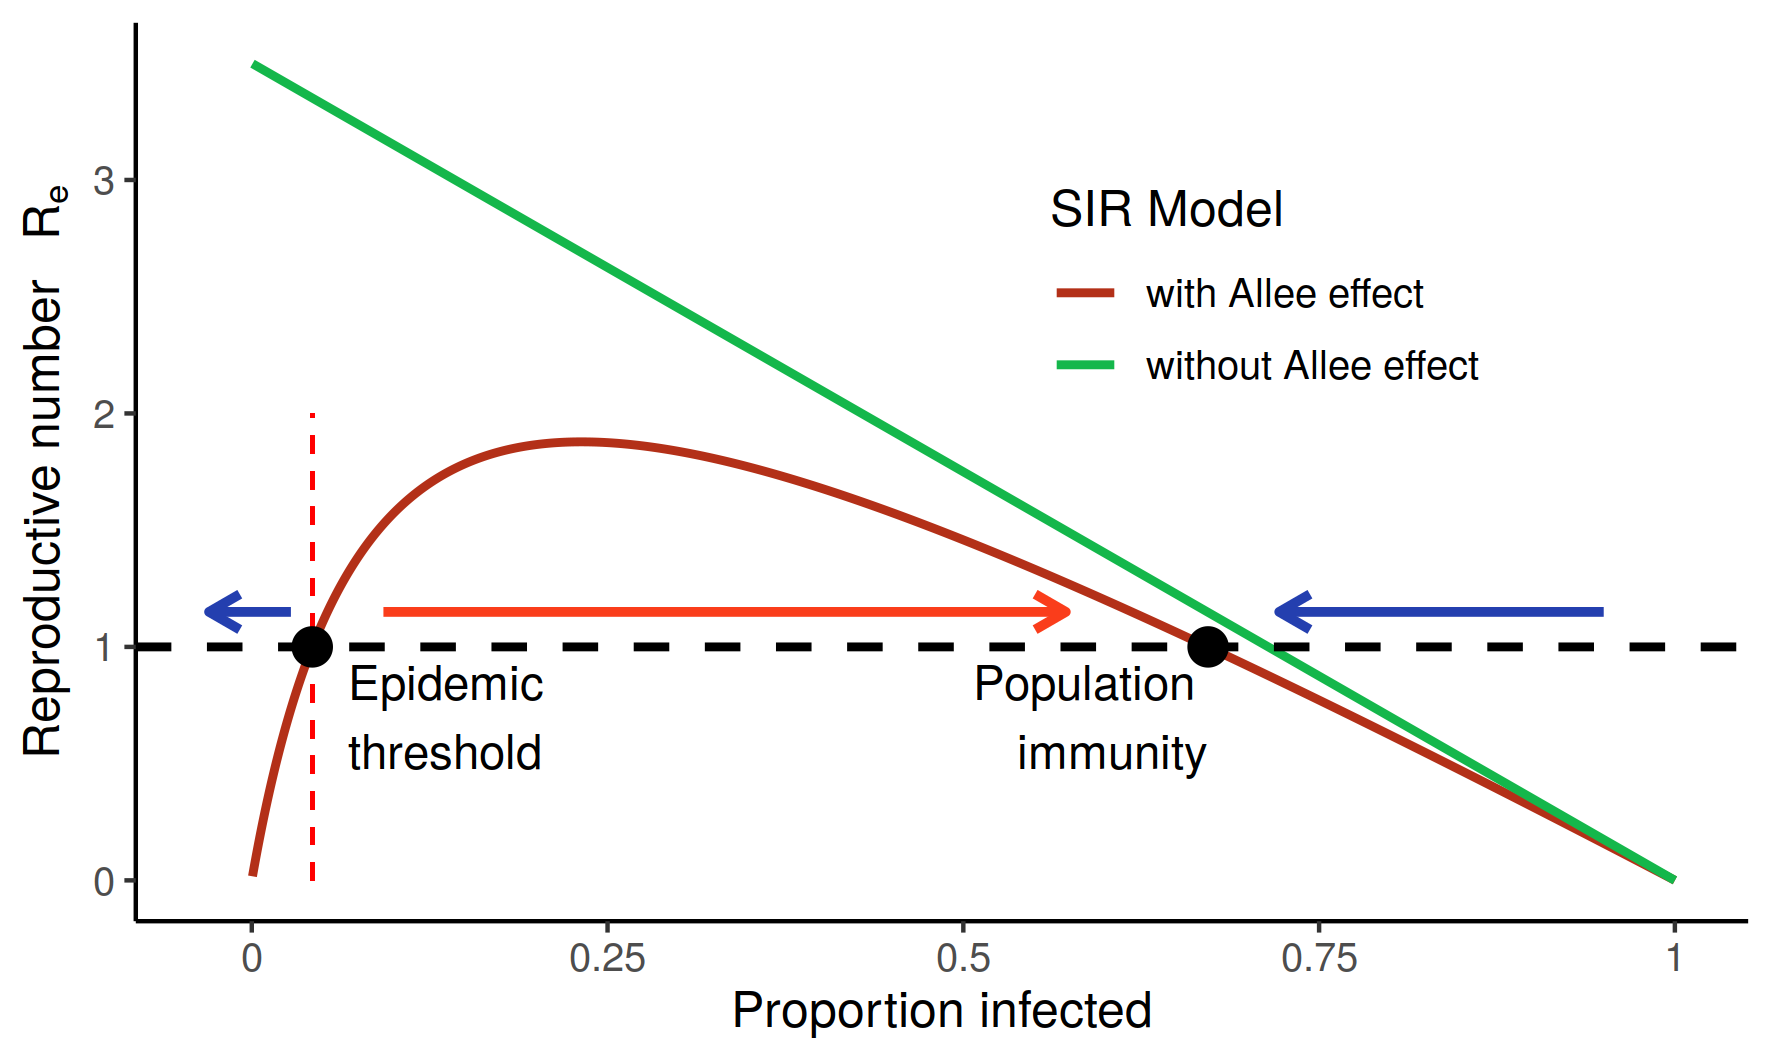
\includegraphics[width=0.6\textwidth]{../allee1D.png}};
   \draw[fill = boxcolor, draw=none]  (\Hone-\BWone,\Vone-\BHone ) rectangle (\Hone+\BWone,\Vone+\BHone)
   

   
    node[pos=0.5] {\scriptsize $Rt = P_{susceptible} \cdot b_{link} (L \cdot f_{c} + L_{max} \cdot f_{nc})$};

   % \draw[fill = blue, draw=none]  (\Htwo-\BWone,\Vone-\BHone ) rectangle (\Htwo+\BWone,\Vone+\BHone)

  \node[anchor=north] at (\Htwo,\Vone) {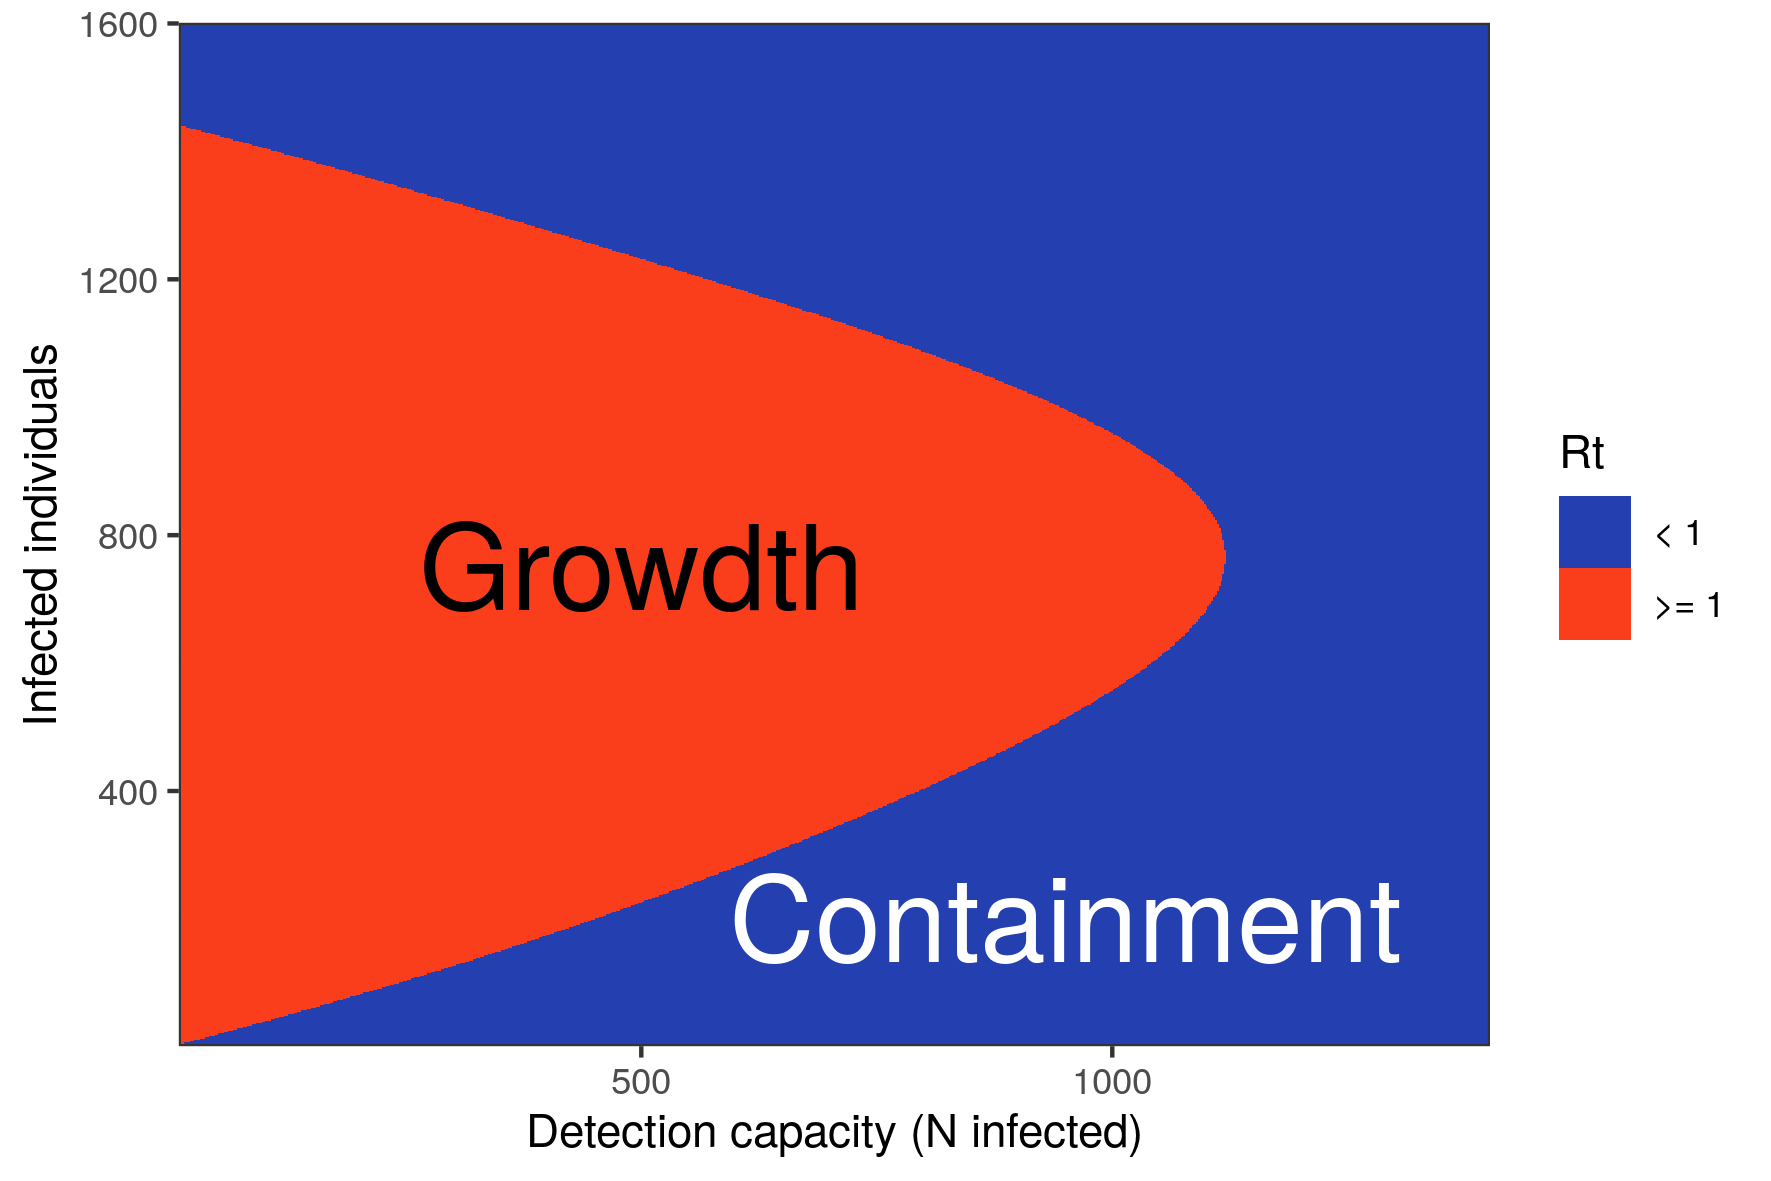
\includegraphics[width=0.55\textwidth]{../phase_space.png}};

  \draw[fill=boxcolor,draw=none]  (\Hone-\BWtwo,\Vtwo-\BHtwo) rectangle (\Hone+\BWtwo+1,\Vtwo+\BHtwo)
    node[pos=0.5,align=left] {\scriptsize  \bf Simulated SIR Dynamics \\
    \scriptsize $\frac{dS}{dt} \sim - \frac{\beta_{max} \cdot I}{I_{50} + I} \cdot I\frac{\cdot S}{N}$ \\
    \scriptsize $\frac{dI}{dt} \sim \frac{\beta_{max} \cdot I}{I_{50} + I} \cdot I\frac{S}{N} - \left(\frac{\gamma_{max} \cdot I}{I_{50} + I}\right)^{-1} \cdot I + NB(\mu,s)$ \\
    \scriptsize $\frac{dR}{dt} \sim - \left(\frac{\gamma_{max} \cdot I}{I_{50} + I}\right)^{-1} \cdot I $};

  \node[anchor=north] at (\Hone+0.5,\Vtwo-1) {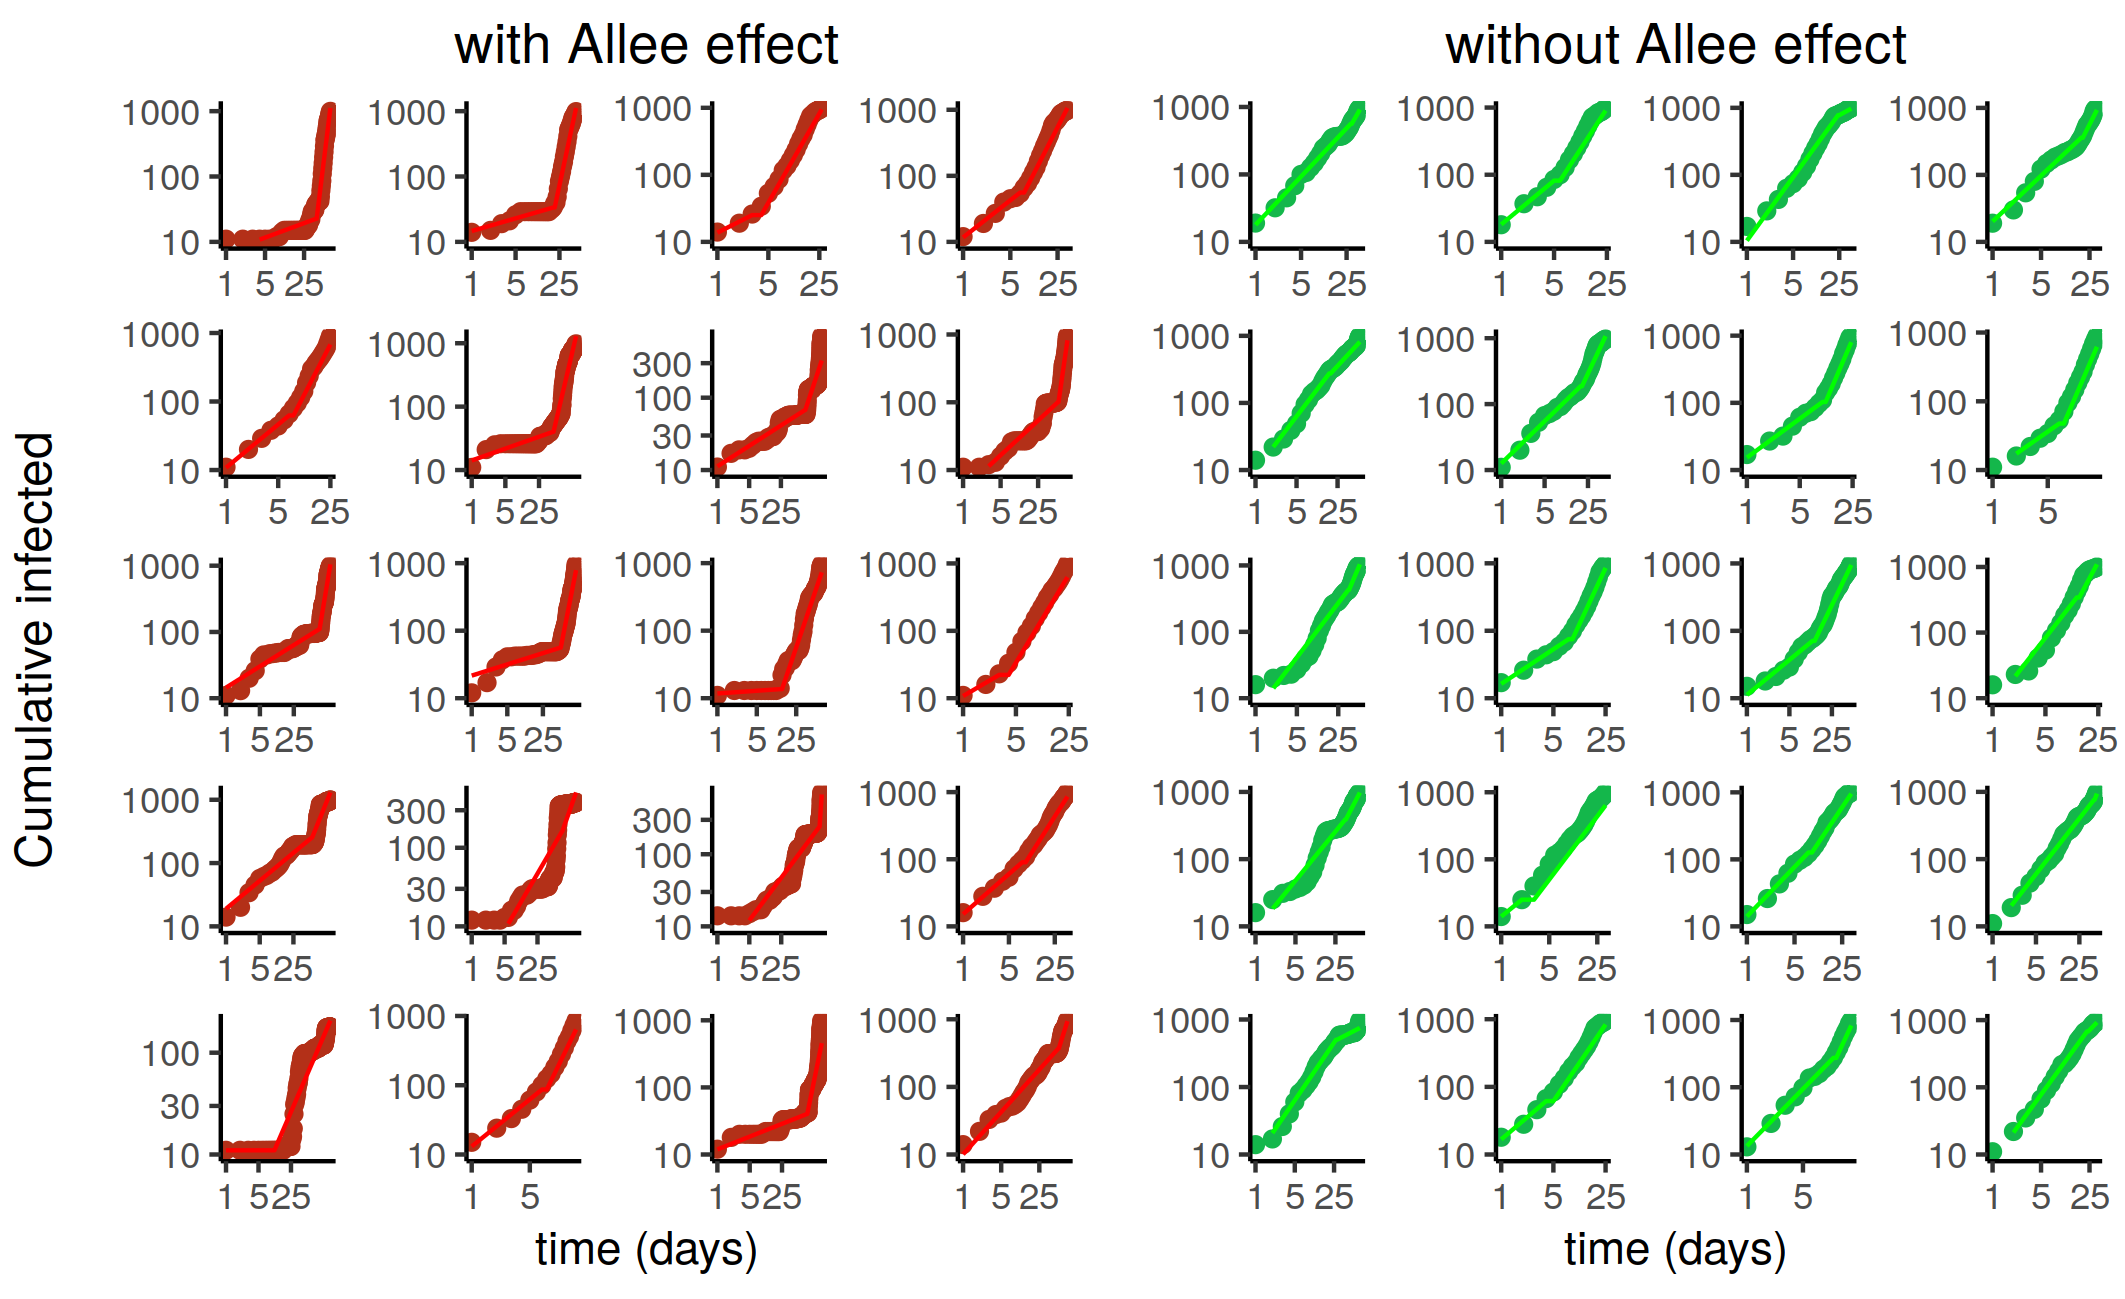
\includegraphics[width=0.68\textwidth]{../simDynamics.png}};

  \node[anchor=north] at (\Htwo+0.5,\Vtwo+1) {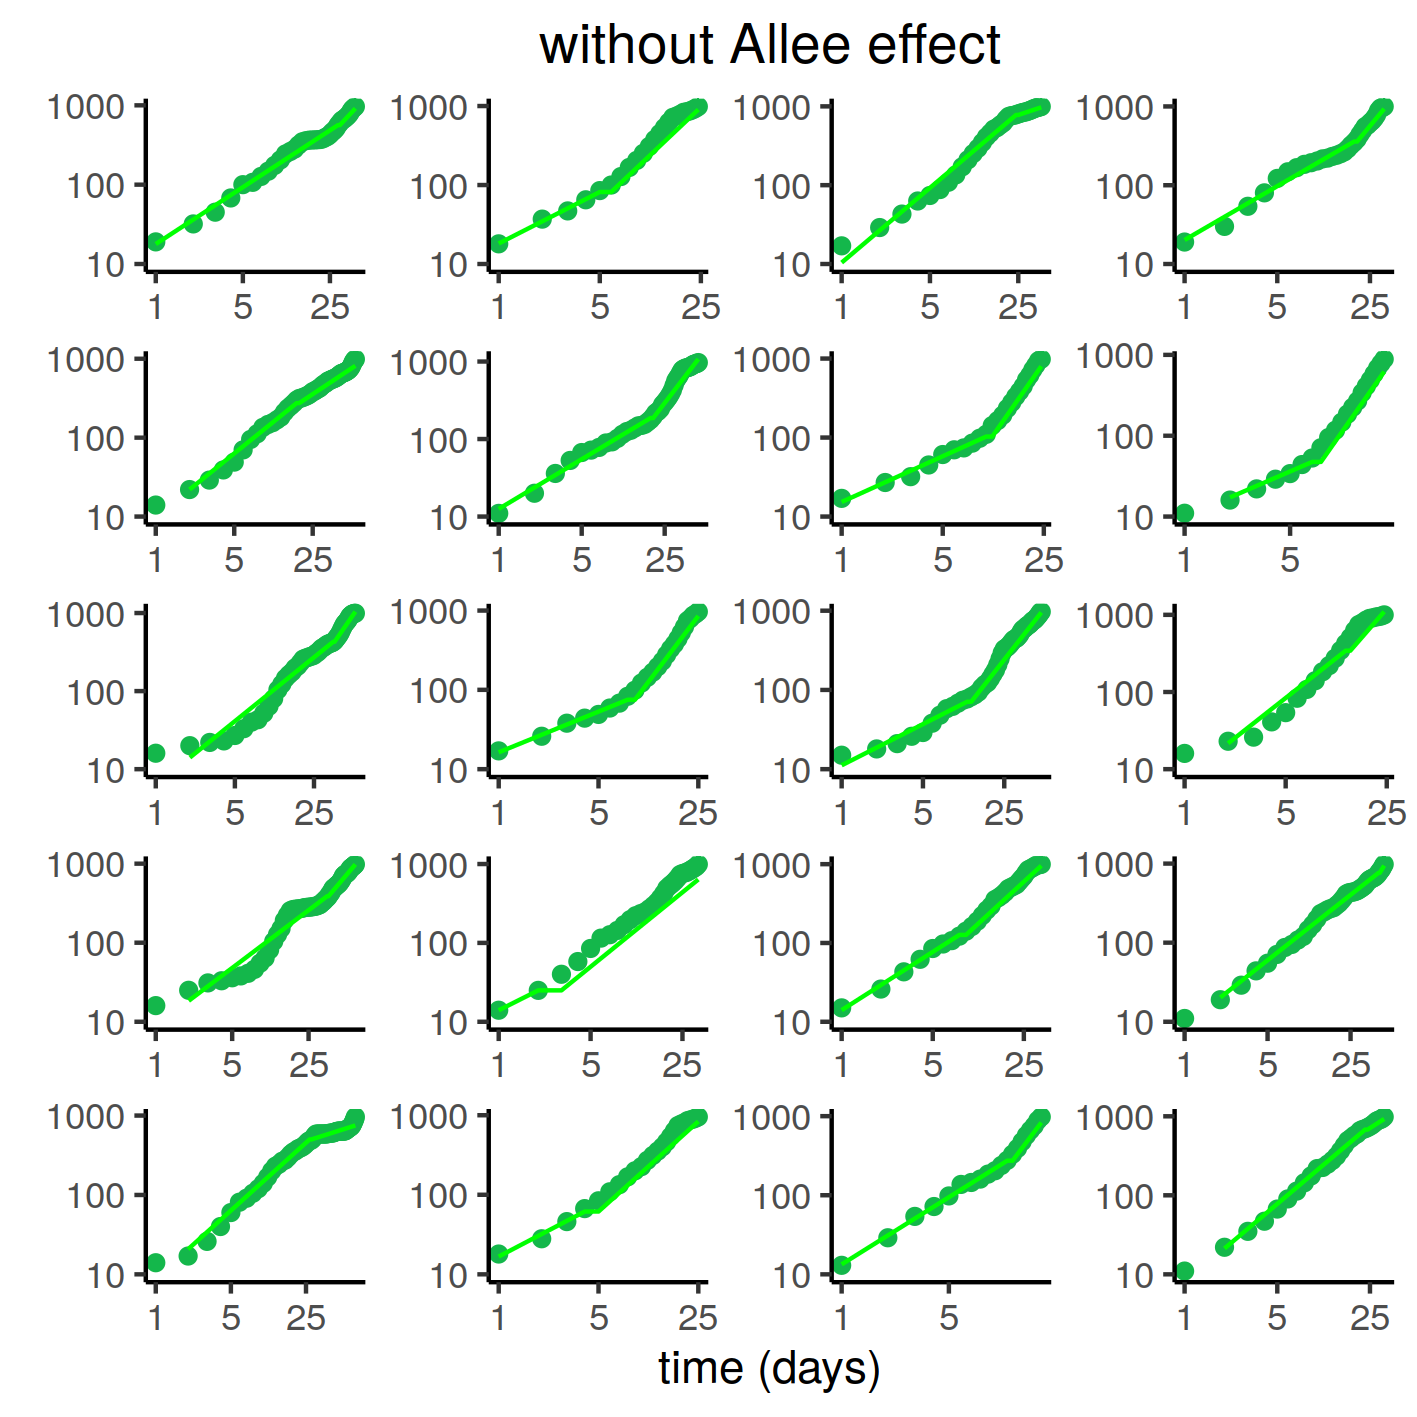
\includegraphics[width=0.6\textwidth]{../slopeAnalysis.png}};


\end{tikzpicture}

\end{adjustwidth}


\end{document}





